\chapter{Problem definition and existing methods of detecting breast cancer}
\label{chap:ch2}

\section{Problem definition}
The problem of detecting breast cancer consists of two main steps: classification and detection. Classification is the process in which, when given an image, the trained model returns a integer value label, representing the class in which the image is predicted to belong to. For the specific problem of detecting breast cancer, a label would take values from 0 to 1, representing normal and cancerous, or to 2, representing cancer, benign and malign. Detection also categorizes the images, but also returns bounding boxes that are predicted to contain the tumor in the image. 

For testing the predictions of a classification model, the most used methods are accuracy, precision and recall, or confusion matrices from which all three values can be calculated from. The formula for these values: \[acc = \frac{TP}{TP + TN + FP + FN},\ precision = \frac{TP}{TP + FP},\ recall = \frac{TP}{TP + FN}\].

The detection model on the other hand, can be tested bu computing IoU, Intersection over Union, that calculates the difference between the predicted image and the true image. For this particular problem, this can be achieved by comparing the original image with the true bounding boxes drawn onto it and the same original image with the predicted bounding boxes drawn. The formula for this metric is: \[IoU = \frac{Area\ of\ overlap}{Area\ of\ union}\].

\section{Databases used in detecting breast cancer}

In the "Existing methods of detecting breast cancer" section of this thesis
I mentioned the WDBC dataset that was used in detecting breast cancer in other research papers. This dataset, also known as Breast Cancer Wisconsin Diagnostic, is found on the website Kaggle, and consists of features extracted from digitized images of a fine needle aspirate, FNA, of a breast mass. The characteristics described, those being ten real values recorded with four significant digits, belong to the cell nuclei found in the images~\cite{link9}. 
Figure \ref{fig:fig28} shows the distribution of the classes among the 569 instances.

\begin{figure}[ht!]
    \centering
    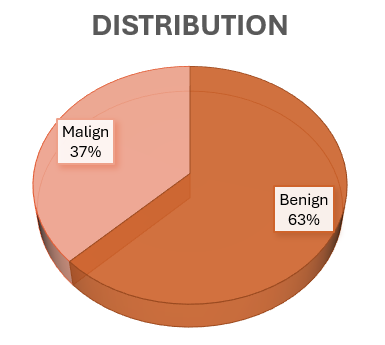
\includegraphics[width=0.5\linewidth]{figures/Figure34.png}
    \caption{Distribution of the classes of the WDBC database among the 569 inputs}
    \label{fig:fig28}
\end{figure}

\begin{figure}[H]
    \centering
    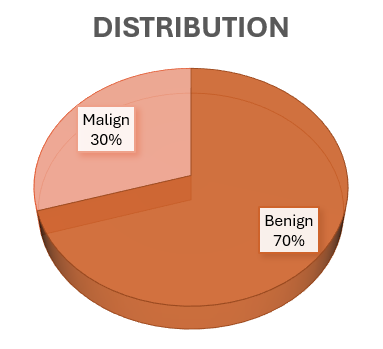
\includegraphics[width=0.5\linewidth]{figures/Figure35.png}
    \caption{Distribution of the classes of the Breast Cancer database among the 286 inputs}
    \label{fig:fig29}
\end{figure}

Other datasets used in breast cancer detection include the Breast Cancer dataset obtained form the University Medical Center, Institute of Oncology, Ljubljana, Yugoslavia. It contains 286 inputs, each with 9 features: class, age, menopause, tumour-size, inv-nodes, node-caps, deg-malig, breast, breast-squad and irradiat~\cite{link10}. Figure \ref{fig:fig29} shows the distribution of the classes.

\section{Existing methods of detecting breast cancer}

There are several articles related to studying various ways of implementing breast cancer detection using machine learning. There is “Machine Learning Techniques for Breast Cancer Prediction” by Varsha Nemade and Vishal Fegade from Mukesh Patel School of Technology Management and Engineering, NMIMS Shirpur Campus, India~\cite{carte2}. They have documented different ML classification techniques and evaluated each of them using different performance measures, such as accuracy, precision, and recall. These techniques include N{\"a}ive Bayes, Logistic Regression, Support Vector Machine, K-Nearest Neighbour and Decision Tree, the latter being found to have the highest accuracy, 97\%. The researchers who conducted this experiment worked with benign and malign classes. 

The dataset used in their experiments was the WDBC dataset, which contains features from 569 digitized images of a fine needle aspirate of a breast mass~\cite{link3}. The algorithm implemented uses features from the image rather than the image itself, some of which include radius, texture, area, perimeter, smoothness, compactness, concavity, concavity points, symmetry and fractal dimension. The following charts represent the performance of the classification techniques used.

\begin{figure}[H]
    \centering
    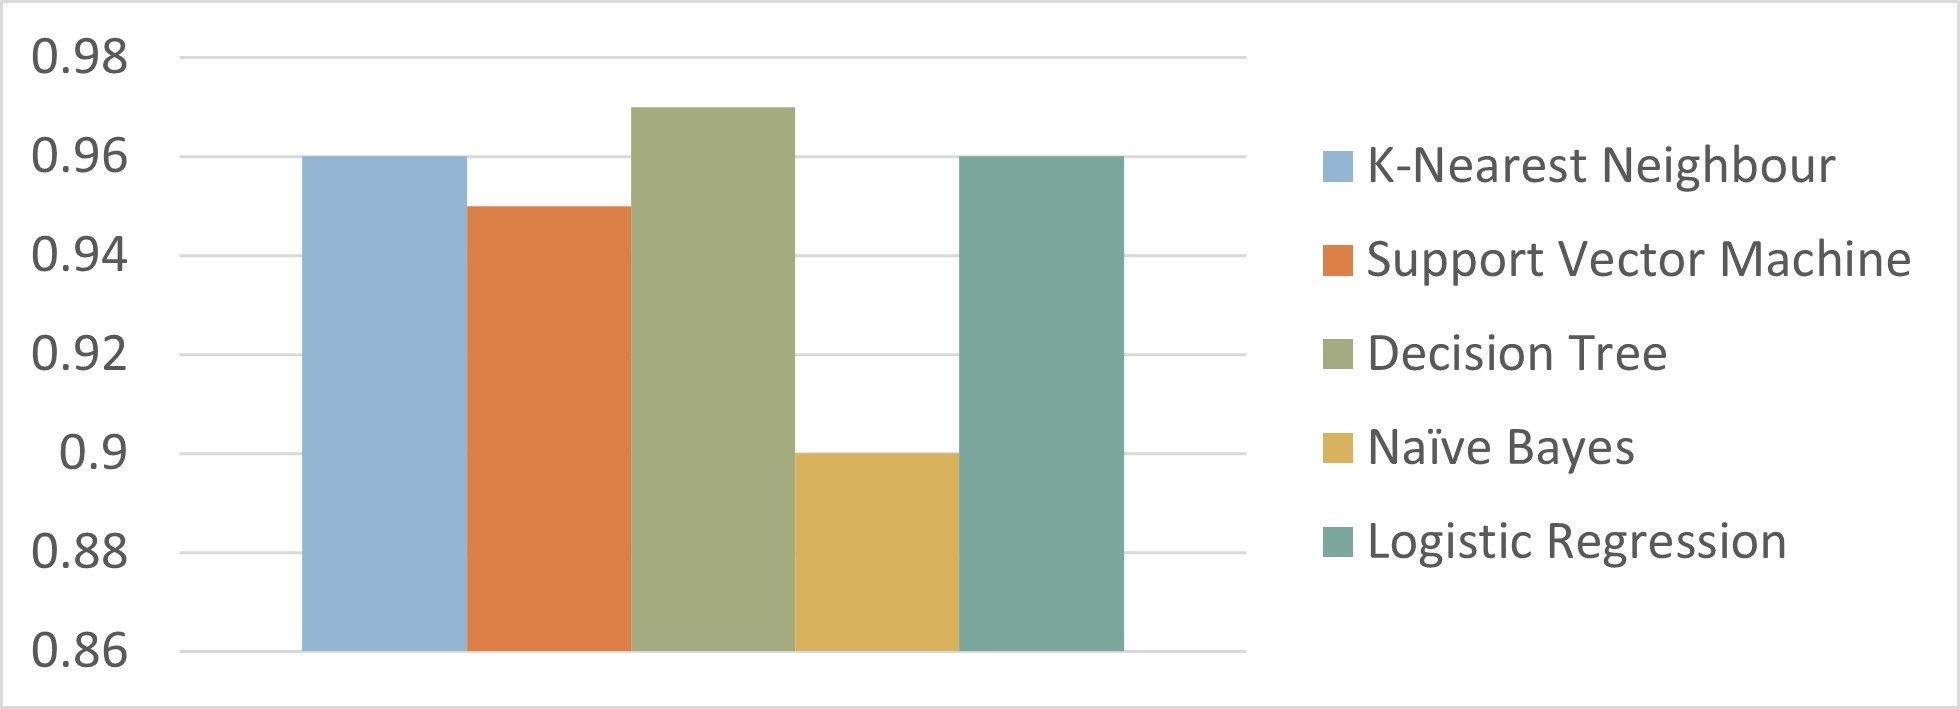
\includegraphics[width=0.75\textwidth]{figures/Figure1.jpg}
    \caption{Accuracy of classification techniques obtained in ~\cite{carte2}}
    \label{fig:fig1}
\end{figure}

\begin{figure}[h!]
    \centering
    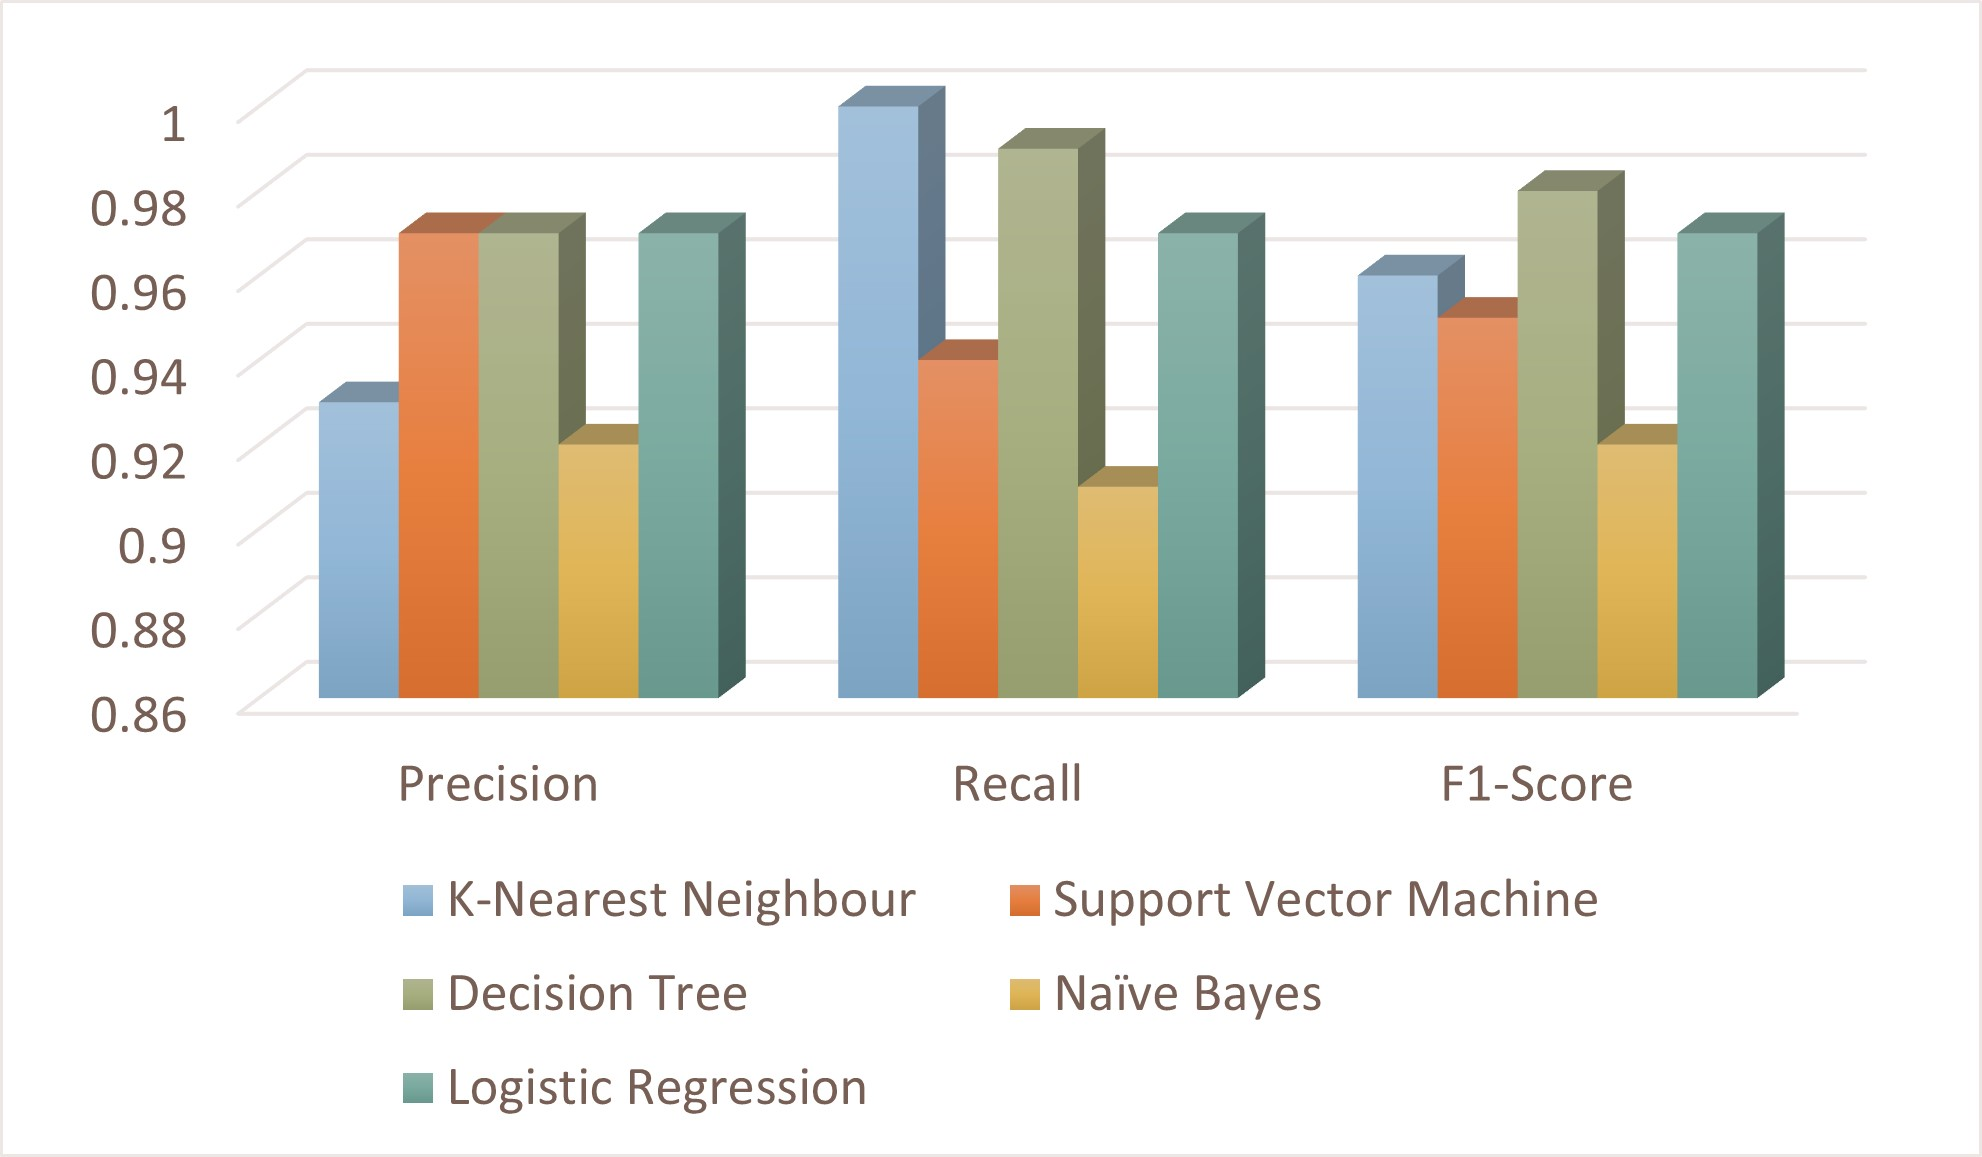
\includegraphics[width=0.75\textwidth]{figures/Figure2.jpg}
    \caption{Performance of classification techniques for class benign obtained in ~\cite{carte2}}
    \label{fig:fig2}
\end{figure}

\begin{figure}[h!]
    \centering
    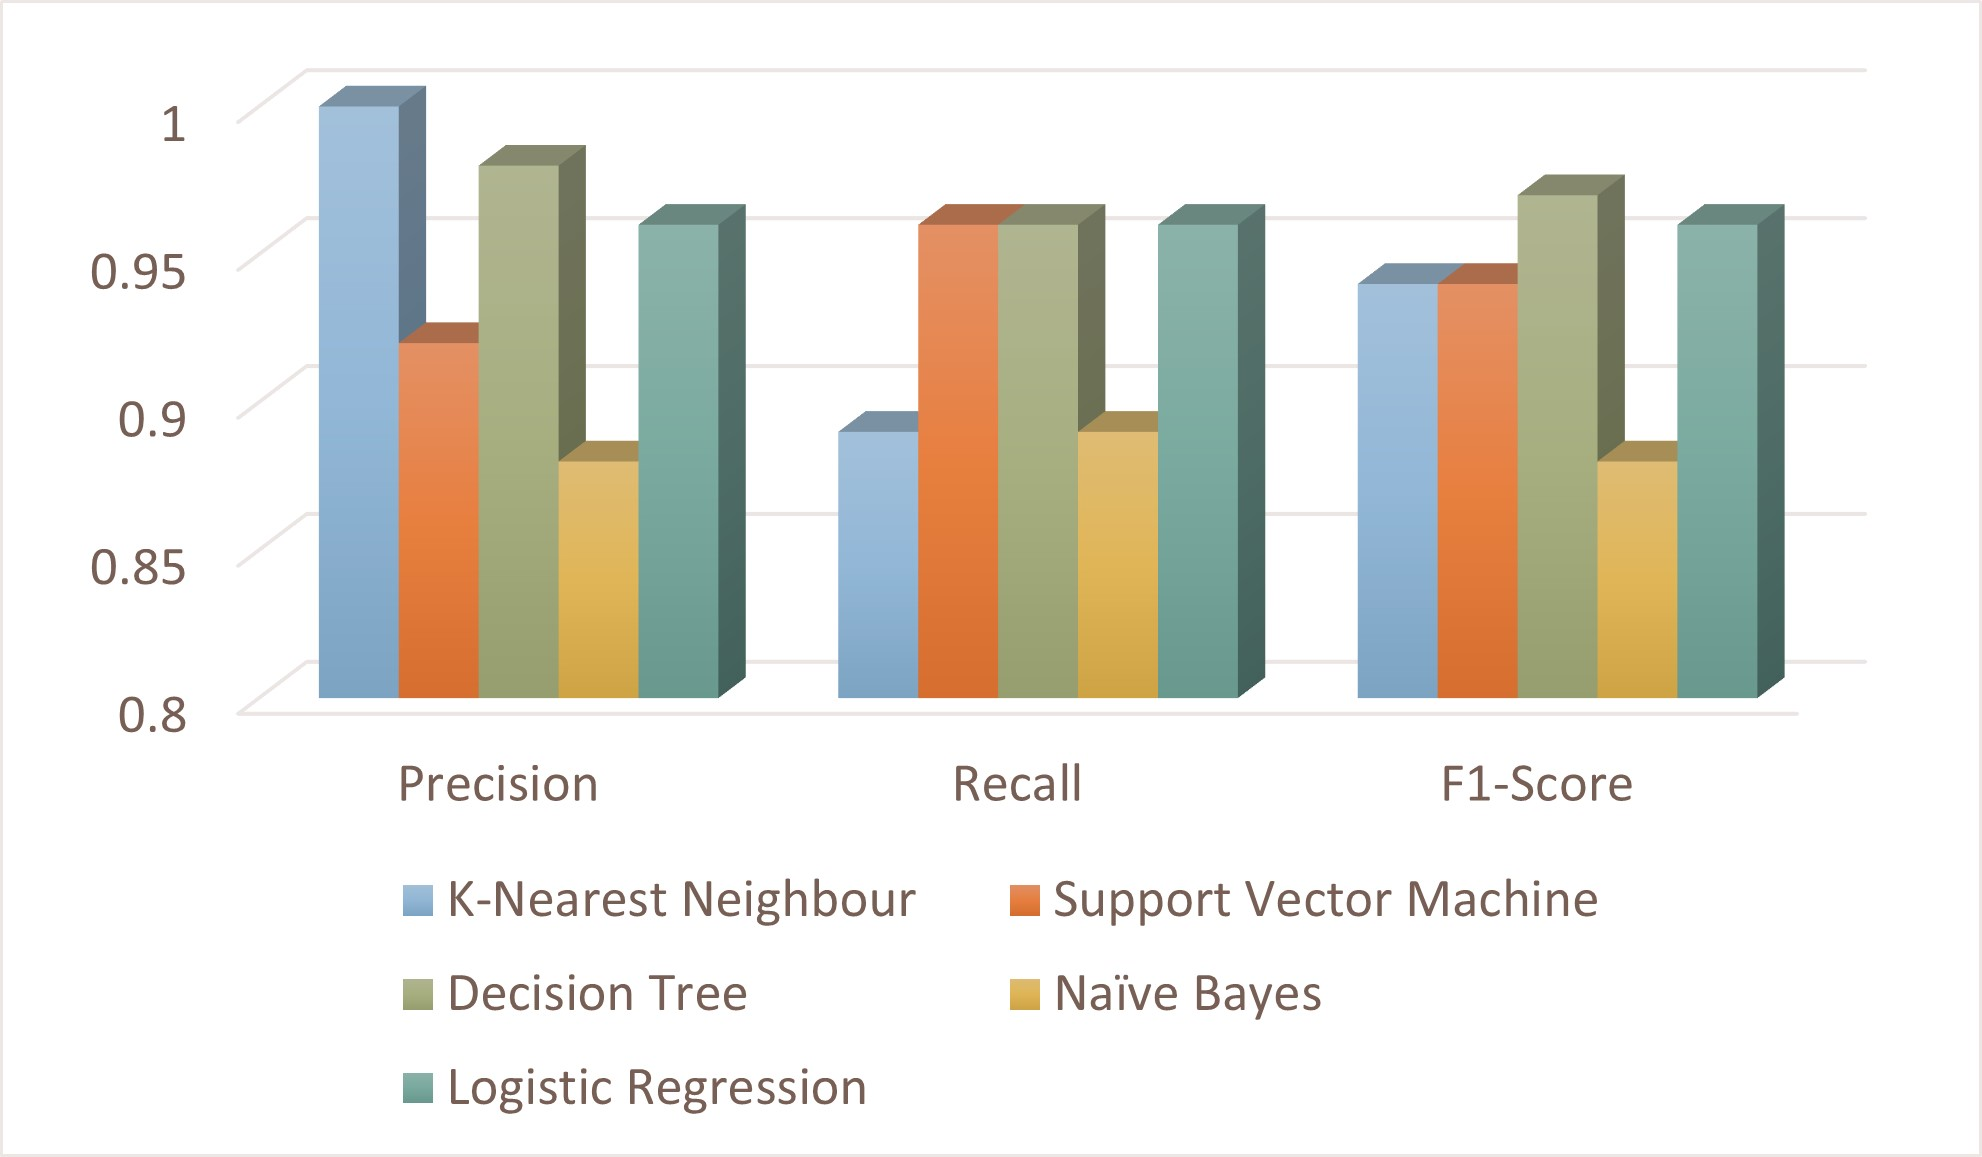
\includegraphics[width=0.75\textwidth]{figures/Figure3.jpg}
    \caption{Performance of classification techniques for class malignant obtained in ~\cite{carte2}}
    \label{fig:fig3}
\end{figure}

Other relevant studies include “An enhanced Predictive heterogeneous ensemble model for breast cancer prediction” concluded by S. Nanglia et al. which got 78\% accuracy using KNN, SVM and DT~\cite{carte1}. Islam et al. got a 98.75\% using ANN on the WDBC~\cite{carte3}. Amrane et al. proposed an approach using KNN and NB with 97.51\% accuracy~\cite{carte4}. Dhahri et al. studied the usage of genetic programming techniques for the selection of the best features and parameters for the machine learning classifier~\cite{carte5}.